\documentclass[12pt,t]{beamer}
\usetheme[greyauthor, % Grå tekst forfatter som KU vil have
         unit=ics, % Ændre til NAT, KU, eller unit=ics (diku)
         dk, % Sprog
         style=simple, % Vandmærke eller billede
         wmark, % vandmærke på hver side
         logoplace=left % Logo til venstre
         %,sidebar % makes sidebar
         ]{Frederiksberg}
% nat for Science, ku for generic or unit=ics for DIKU
% Tilføj style=simple for vandmærke

\usepackage{pslatex} % pæn skrift
\usepackage[utf8]{inputenc} % Implementerer Unicode
\usepackage{graphicx}
\usepackage{float}
\usepackage{listings}

\title{Programmeringssprog}
\subtitle{Datalogens Værktøj}
\author{
        Arinbjörn Brandsson - Arbr@di.ku.dk \\
        Benjamin Rotendahl - Bero@di.ku.dk\\
        Mathias Mortensen - Mamo@di.ku.dk
}

\date[]{\today}

\begin{document}
\frame[nat]{\titlepage}

\begin{frame}
\frametitle{Hvad er Programmeringssprog?}
\begin{block}{Et Værktøj}
\begin{itemize}
\item Programmeringssprog bruges som et værktøj til at løse en problemstilling\\
\item Forskellige programmeringssprog bruges til forskellige formål
\end{itemize}
\end{block}
\begin{block}{Et Regelsæt til Hvordan der Kommunikeres}
\begin{itemize}
\item Et programmeringssprog definerer hvordan man \textbf{kan} kommunikere med 
en datamat\\
\item Uden programmeringssprog skulle vi kode i maskinssprog
\end{itemize}
\end{block}
\end{frame}

\begin{frame}
\frametitle{Opbygning af et Programmeringssprog}
\begin{block}{Hvordan Kan Datamater Forstå Programmeringssprog?}
\begin{itemize}
\item Programmeringssproget checkes for syntaksfejl\\
\item Derefter køres den igennem dens sprog-specifikke oversætter, 
som oversætter koden til MIPS Assembly (Maskinsprog for mennesker)\\
\item MIPS Assembly oversættes af datamaten om til binært som den kan forstå
\end{itemize}
\end{block}
\end{frame}

\begin{frame}
\begin{figure}[h]
\centering
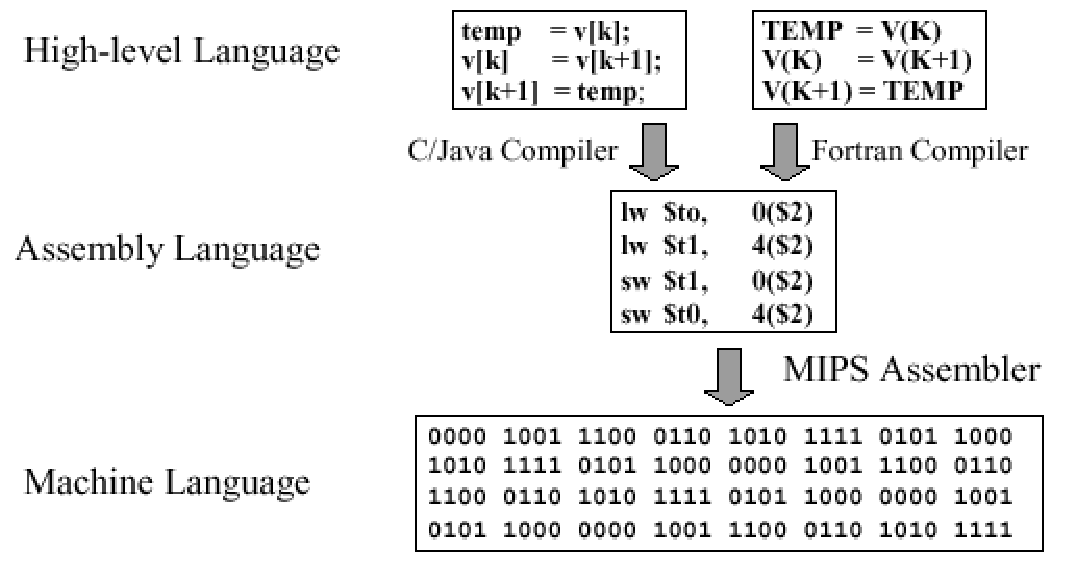
\includegraphics[scale=0.55]{Img/LangToMachine.pdf}
\end{figure}
\end{frame}
\begin{frame}
\frametitle{Turing Tarpit}
"Beware of the Turing tar-pit in which everything is possible but nothing of interest is easy."\\
~~~~~~~~~~-Alan Perlis, \emph{Epigrams on Programming}\\
\begin{block}{Turing Komplethed}
Et programmeringssprog er Turing komplet hvis alle (korrekte) algoritmer kan 
køres ved brug af programmeringssproget
\end{block}
\end{frame}
\begin{frame}[fragile]
\frametitle{Turing Tarpit Eksempel}
Eksempel: "Hello, World!" i \texttt{Brainfuck}\pause
\begin{lstlisting}[basicstyle=\tiny]
+++++ +++               Set Cell #0 to 8
[
    >++++               Add 4 to Cell #1; this will always set Cell #1 to 4
    [                   as the cell will be cleared by the loop
        >++             Add 2 to Cell #2
        >+++            Add 3 to Cell #3
        >+++            Add 3 to Cell #4
        >+              Add 1 to Cell #5
        <<<<-           Decrement the loop counter in Cell #1
    ]                   Loop till Cell #1 is zero; number of iterations is 4
    >+                  Add 1 to Cell #2
    >+                  Add 1 to Cell #3
    >-                  Subtract 1 from Cell #4
    >>+                 Add 1 to Cell #6
    [<]                 Move back to the first zero cell you find; this will
                        be Cell #1 which was cleared by the previous loop
    <-                  Decrement the loop Counter in Cell #0
]                       Loop till Cell #0 is zero; number of iterations is 8
>>.                     Cell #2 has value 72 which is 'H'
>---.                   Subtract 3 from Cell #3 to get 101 which is 'e'
+++++++..+++.           Likewise for 'llo' from Cell #3
>>.                     Cell #5 is 32 for the space
<-.                     Subtract 1 from Cell #4 for 87 to give a 'W'
<.                      Cell #3 was set to 'o' from the end of 'Hello'
+++.------.--------.    Cell #3 for 'rl' and 'd'
>>+.                    Add 1 to Cell #5 gives us an exclamation point
>++.                    And finally a newline from Cell #6
\end{lstlisting}
\end{frame}

\begin{frame}[fragile]
\frametitle{Turing Tarpit - Fortsat}
"Hello, World!" i C:\pause
\begin{lstlisting}[language=C]
#include<stdio.h>

main()
{
    printf("Hello, World");

}
\end{lstlisting}
\end{frame}

\begin{frame}
 \frametitle{Krav til et Godt Programmeringssprog}
 \begin{block}{}
  \begin{itemize}
  \item Skal være læsbart og forståeligt\\
  \item Programmeringssprogets syntaks må ikke lede til tvetydigheder
  \begin{itemize} 
  \item For eksempel må der ikke være forvirring over hvad resultatet af "2+4/2" er
  \end{itemize}
  \item Skal have dokumentation over hvordan programmeringssproget virker og er 
  struktureret
  \end{itemize}
 \end{block}
\end{frame}

\begin{frame}
 \frametitle{Programmeringssprogstyper {\tiny (Imperative \& Declarative)}}
 \begin{block}{Der Findes Mange Forskellige Typer af Programmeringssprog}
 \begin{itemize}
  \item Object-Orientered programming
  \item Functional programming, og
  \item Logic programming
 \end{itemize}
 \end{block}
 \begin{exampleblock}{Og Disse Kan Underklassificeres}
 \begin{itemize}
 \item Static/Dynamic typing
 \item Weak/Strong typing
 \item High-level/Low-level, og flere!
 \end{itemize}
 \end{exampleblock}
 Disse beskrivelser af et programmeringssprog kaldes for paradigmer
\end{frame}

\begin{frame}
\frametitle{Object-Oriented Programming}
\begin{block}{Klasser og Objekter}
\begin{itemize}
\item Klasse: Man definere et skelet for fremtidige versioner\\
\begin{itemize}
\item Eksempel: Et menneske har to arme, to ben, øjne og hår
\end{itemize} 
\item Objekt: Man instantiere skelettet med værdier man selv bestemmer\\
\begin{itemize}
\item Eksempel: Et menneske har brune øjne, og sort hår
\end{itemize}
\end{itemize}
\end{block}
\begin{block}{}
Kan bruges til mange forskellige ting, som for eksempel hvis der er brug for 
en grafisk overflade som kan manipuleres
\end{block}
\end{frame}

\begin{frame}[fragile]
\frametitle{Notable Example}
\begin{block}{Java}
\begin{itemize}
\item Nem at lære
\item Kan bruges på alle platforme via virtual machines (skalerbart)
\item Har utrolig meget support
\end{itemize}
\end{block}
\begin{lstlisting}[language=Java]
public class HelloWorld {
    public static void main(String[] args) {
        // Prints "Hello, World" to the terminal.
        System.out.println("Hello, World");
    }
}

\end{lstlisting}
\end{frame}

\begin{frame}
\frametitle{Functional Programming}
\begin{block}{Funktioner og Deling}
\begin{itemize}
\item En funktions output er kun afhængig af dens input
\item Kan (typisk) beskrive det samme som i et objekt-orienteret sprog i 
færre linjer
\item Er industri standard i matematisk analyse, (nogen typer) machine learning, 
text redigering og analyse, og noget back-end
\end{itemize}
\end{block}
\end{frame}

\begin{frame}[fragile]
\frametitle{Notable Example}
\begin{block}{Haskell}
\begin{itemize}
\item Industri-standard funktionel programmeringssprog grundet monader
\item Nemt at lære, svær at mestre
\end{itemize}
\end{block}
\begin{lstlisting}[language=Haskell]
main = putStrLn "Hello, World!"
\end{lstlisting}
\end{frame}

%Prolog!
\begin{frame}
\frametitle{Logic Programming}
\begin{block}{Logik med Logik På}
\begin{itemize}
\item Bruges til at finde en (eller flere) sandhedsværdier i et input
\item Kan bruges til AI, for eksempel
\end{itemize}
\end{block}
\end{frame}

\begin{frame}[fragile]
\frametitle{Notable Example}
\begin{block}{ProLog}
\begin{itemize}
\item Er specialiseret til bruger defineret logik relationer
\end{itemize}
\end{block}
\begin{lstlisting}{language=ProLog}
:- initialization(main).
main :- write('Hello World!'), nl, halt.
\end{lstlisting}
\end{frame}
% \begin{frame}
%   \frametitle{Søgning}
%   \begin{block}{Mål}
%   Givet en sorteret liste, find så et specifikt element ved at kigge på så få elementer som muligt.
%   \end{block}
%   \pause

%   \begin{exampleblock}{Eksempel}
%   Lad en liste være givet ved $[2, 4, 5, 7, 8, 11, 25]$, hvor vi ønsker at finde indeks for elementet 11. Svaret skulle gerne være 5 (det første element har indeks 0).
%   \end{exampleblock}
% \end{frame}

% \begin{frame}
%   \frametitle{Sortering}
%   \begin{block}{Mål}
%   Sorter en givet usorteret liste.
%   \end{block}
%   \pause

%   \begin{exampleblock}{Eksempel}
%   Lad en liste være givet ved [7, 4, 5, 12, 1], denne vil vi gerne sortere! Den sorterede liste skulle gerne være [1, 4, 5, 7, 12].
%   \end{exampleblock}
% \end{frame}

% \begin{frame}
%   \frametitle{Implementering af sorteringsmetode}
%   \begin{block}{Mål}
%   Skriv en algoritme for Bubble Sort.
%   \end{block}
%   \pause

%   \begin{exampleblock}{Eksempel}
%   Tavledemonstration!
%   \end{exampleblock}
% \end{frame}

% \begin{frame}{Primtal}
%   \begin{block}{Mål}
%   Skriv en algoritme der finder det $n$'te primtal - prøv at gør den så hurtig som mulig.
%   \end{block}
%   \pause

%   \begin{exampleblock}{Eksempel}
%   Find det femte primtal. Algortimen skal gerne returnere 11.
%   \end{exampleblock}
% \end{frame}

\end{document}